
\section{PL/SQL}
\subsection{Introduction}
\begin{tcolorbox}[title = Definition]
PL/SQL, or Procedural Language/Structured Query Language, is an extension of SQL. While SQL (Structured Query Language) is primarily used for CRUD operations (querying, inserting, updating, and deleting data in relational databases), PL/SQL allows for full programmatic control with features such as control structures (loops and conditionals), variables, and error handling with exceptions. This enables the creation of scripts that can automate tasks with functions, procedures, and triggers, implement complex business logic, and manipulate data at a higher level than SQL alone.
\end{tcolorbox}

\begin{tcolorbox}[title = Differences Between PL/SQL and SQL]
\begin{itemize}
    \item SQL is limited to CRUD operations; PL/SQL adds procedural programming capabilities.
    \item PL/SQL provides advanced error handling through exceptions.
    \item PL/SQL supports modular programming with functions, procedures, and triggers.
    \item PL/SQL is specific to Oracle databases, whereas SQL is standardized across various databases.
\end{itemize} 
\end{tcolorbox}

\subsection{Overview Of Plsql's Structure}
\begin{tcolorbox}[title = Programme Structure]
A PL/SQL has 3 blocks :
\begin{itemize}
    \item DECLARE(Optional Block) : contains all the declared variables , constants \& modules(functions,procedure) 
    \item MAIN : contains the main executable code 
    \item EXCEPTION(Optional Block) : handls erros with exceptions 
\end{itemize}
\end{tcolorbox}
\begin{center}
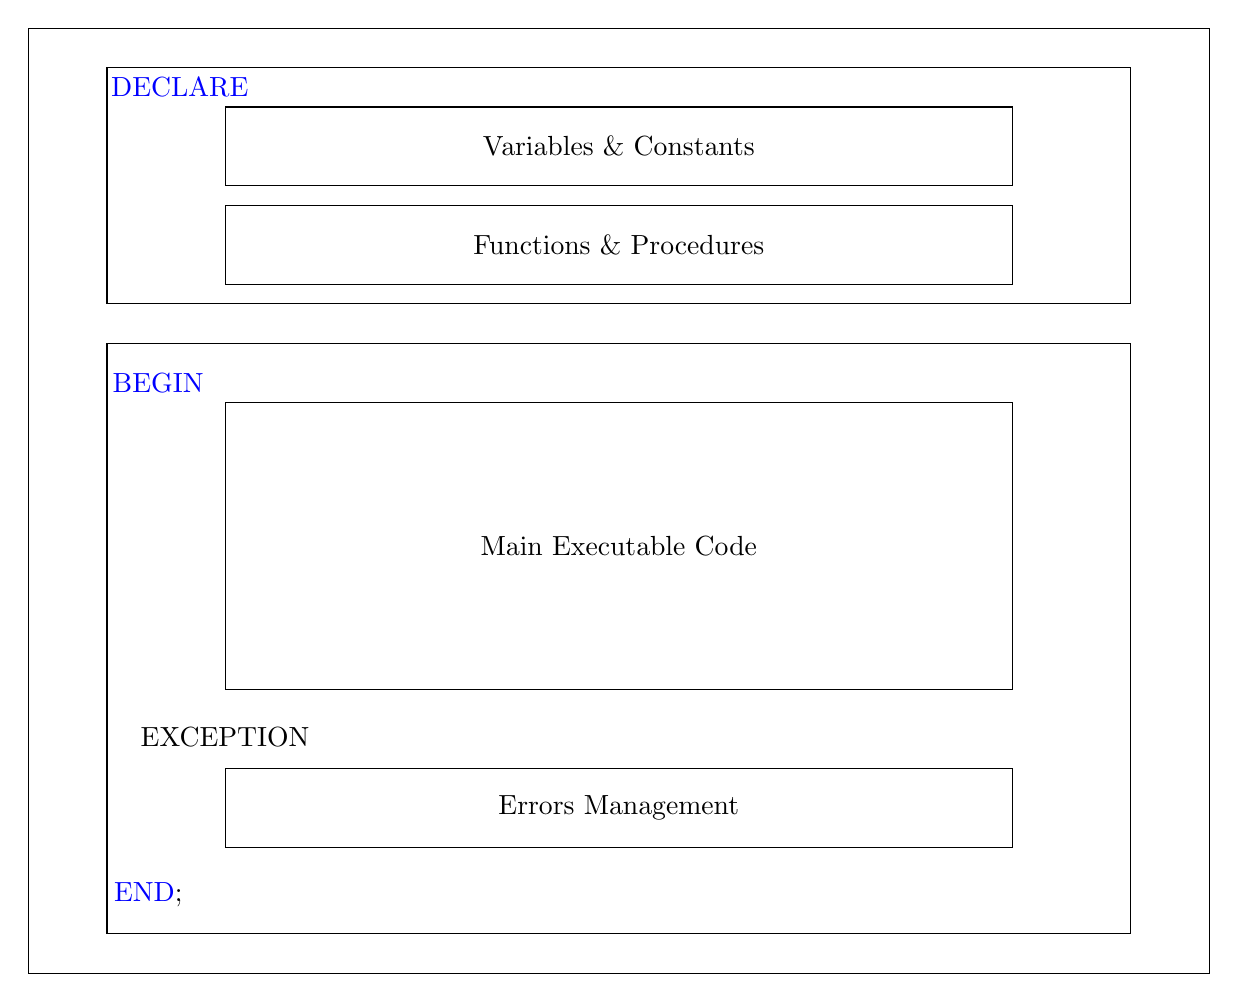
\begin{tikzpicture}
    \draw (0,0) rectangle (15,12);
    
    \draw (1,8.5) rectangle(14,11.5);
    \node at (1.925,11.25) {\textcolor{blue}{DECLARE}};
    \draw (2.5,10) rectangle (12.5,11);
    \node at(7.5,10.5){Variables \& Constants};
    \draw (2.5,8.75) rectangle (12.5,9.75);
    \node at (7.5,9.25){Functions \& Procedures};
    
    \draw (1,0.5) rectangle(14,8);
    \node at (1.65,7.5) {\textcolor{blue}{BEGIN}};
    \draw (2.5,3.6) rectangle (12.5,7.25);
    \node at (7.5,5.425){Main Executable Code};
    \node at (2.5,3) {EXCEPTION};
    \draw (2.5,1.6) rectangle (12.5,2.6);
    \node at (7.5,2.1){Errors Management};
    \node at (1.525,1) {\textcolor{blue}{END};};
\end{tikzpicture}
\end{center}
\subsection{Comments}
\begin{tcolorbox}[title  = Comments Syntax]
\textbf{\underline{One Line Comment}:}

\vspace{0.25cm}
\textcolor{commentgray}{- - Comment here}

\vspace{0.25cm}
\textbf{\underline{Multiple Lines Comment}:}

\vspace{0.25cm}
\textcolor{commentgray}{/*\\
This is a Mulitple\\
Lines Comment\\
*/}
\end{tcolorbox}


\subsection{Printing}
\begin{tcolorbox}[title = DBMS\_OUTPUT.PUT\_LINE]
To print messages in the console, we use the \texttt{DBMS\_OUTPUT.PUT\_LINE} command. The message should be enclosed
in single quotes ' ' and we use double pipes \texttt{||} to concatenate with variables:

\begin{center}
DBMS\_OUTPUT.PUT\_LINE(\textcolor{messagegreen}{'Hello '} \texttt{||} name \texttt{||} \textcolor{messagegreen}{'!'} );
\end{center}
\end{tcolorbox}

\begin{tcolorbox}[title = Note]
To be able to see the printed messages in the console of SQL*Plus, SQL Developer, etc., we need to activate
the buffer responsible for printing the messages by using the command: 
\begin{center}
    \textcolor{blue}{SET} SERVEROUTPUT \textcolor{blue}{ON};
\end{center}
Note that this is only needed once , and it will remain active unless you explicitly turn it off.
\end{tcolorbox}
\subsection{Variables Declaration \& Types}
\begin{tcolorbox}[title = Variables \& Constants]
All variables and constants must be declared in the \textcolor{blue}{DECLARE} scope the syntax is as follows

\vspace{0.35cm}

\hspace{4cm}varName dataType := value\hspace{3.95cm}\textcolor{commentgray}{- - Variable Declaration}

\vspace {0.15cm}
\hspace{4cm}constName CONSTANT dataType := value\hspace{1.5cm}\textcolor{commentgray}{- - Constant Declaration}\\

\end{tcolorbox}

\begin{tcolorbox}[title = Types]
PL/SQL supports many standard data types, as seen previously. Here, we introduce two additional types:

\begin{itemize}
    \item \textbf{Type:} Used to define a variable with the same data type as a column in a table:
        \begin{center}
            varName tableName.columnName\%TYPE;
        \end{center}
    \item \textbf{RowType:} Used to define a variable as a record with the structure of a row in a table:
        \begin{center}
            varName tableName\%ROWTYPE;
        \end{center}
\end{itemize}

\end{tcolorbox}



\begin{tcolorbox}[title = Store Select Output In Variables]
We can store the output of the \textcolor{blue}{SELECT} command in variables using the \textcolor{blue}{INTO} clause as follows:

\begin{center}
\textcolor{blue}{SELECT} col$_{1}$, col$_{2}$, ..., col$_{n}$ 
\textcolor{blue}{INTO} var$_{1}$, var$_{2}$, ..., var$_{n}$ 
\textcolor{blue}{FROM} tableName 
\textcolor{blue}{WHERE} [conditions];
\end{center}

\end{tcolorbox}
\begin{tcolorbox}[title = Note]
\textbf{\underline{Order Of Variables Is Important}}

The order of the variables in the \textcolor{blue}{INTO} clause must match the order of the selected columns

\textbf{\underline{Select Should Ouput One Line Only}}

When Storing the output of \textcolor{blue}{SELECT} in variables , the ouput should be one line and not a table
if not we will have to use cursor to navigate through the table we will cover that later on
\end{tcolorbox}
\subsection{Control Structures}
\begin{tcolorbox}[title = Definition]
In PL/SQL, control structures are constructs that help control the flow of execution in a block of code.
They determine the order and conditions under which statements are executed and help make the code dynamic
and responsive to varying conditions. The main types of control structures in PL/SQL are:
\end{tcolorbox}
\subsubsection{Conditional Control}
\begin{tcolorbox}[title = If] 

    \textcolor{blue}{IF} condition1 \textcolor{blue}{THEN}

    \textcolor{commentgray}{- - statements to execute if condition1 is true}

    \textcolor{blue}{ELSIF} condition2 \textcolor{blue}{THEN}

    \textcolor{commentgray}{- - statements to execute if condition2 is true}

    \textcolor{blue}{ELSE}

    \textcolor{commentgray}{- - statements to execute if none of the conditions are true}

   \textcolor{blue}{END IF};
\end{tcolorbox}
\begin{tcolorbox}[title = Switch Case]
    
\textcolor{blue}{CASE} \\
\textcolor{blue}{WHEN} condition1 \textcolor{blue}{THEN}\\
\textcolor{commentgray}{- - statements to execute if condition1 is true}\\
\textcolor{blue}{WHEN} condition2 \textcolor{blue}{THEN}\\
\textcolor{commentgray}{- - statements to execute if condition2 is true}\\
        \textcolor{blue}{ELSE}\\
        \textcolor{commentgray}{- - statements to execute if none of the conditions are true}\\
\textcolor{blue}{END CASE};

\end{tcolorbox}
\subsubsection{Looping Control}
\begin{tcolorbox}[title = Simple Loop] 

LOOP\\
    \textcolor{commentgray}{- - statements to execute}\\
    EXIT \textcolor{blue}{WHEN} condition; \textcolor{commentgray}{- - condition to exit the loop}\\
\textcolor{blue}{END} LOOP;
\end{tcolorbox}
\begin{tcolorbox}[title = While Loop]
WHILE condition LOOP\\
\textcolor{commentgray}{- - statements to execute while condition is true}\\
\textcolor{blue}{END} LOOP;
\end{tcolorbox}
\begin{tcolorbox}[title = For Loop]
 \textbf{Ascending}

\vspace{0.15cm}
\textcolor{blue}{FOR} counter \textcolor{blue}{IN} start..end LOOP\\
\textcolor {commentgray}{- - statements to execute for each value of counter}\\
\textcolor{blue}{END} LOOP;

\vspace{0.25cm}
 \textbf{Descending}

 \vspace{0.15cm} 
\textcolor{blue}{FOR} counter \textcolor{blue}{IN} REVERSE end..start LOOP\\
\textcolor {commentgray}{- - statements to execute for each value of counter}\\
\textcolor{blue}{END} LOOP;

\end{tcolorbox}
\subsection{Raise Application Error}
\begin{tcolorbox}[title = Raise Errors] 
RAISE\_APPLICATION\_ERROR is a procedure used to raise an error that halts code execution, with a custom error
message. Each error\_code (between -20000 and -20999) is associated with an error message retrieved 
by SQLERRM, while SQLCODE captures the error code itself.

\begin{center}
RAISE\_APPLICATION\_ERROR(error\_code, error\_message);
\end{center}

Though commonly used to handle user-defined exceptions, RAISE\_APPLICATION\_ERROR can also be used internally
by the system for predefined exceptions, supporting error control in both system and custom PL/SQL operations.
\end{tcolorbox}


\subsection{Exceptions}
\begin{tcolorbox}[title = Definition]
Exceptions help manage errors and improve readability compared to directly using RAISE\_APPLICATION\_ERROR. Under
the hood, exceptions are built on RAISE\_APPLICATION\_ERROR. There are two main types of exceptions:
\begin{itemize}
    \item \textbf{Predefined Exceptions}: These are system-defined exceptions, such as:
        \begin{itemize}
            \item NO\_DATA\_FOUND: Raised when a \textcolor{blue}{SELECT} statement returns no rows.
            \item TOO\_MANY\_ROWS: Raised when a \textcolor{blue}{SELECT} statement returns more than one row.
        \end{itemize}
    \item \textbf{User-defined Exceptions}: Defined by the user using the \textcolor{blue}{EXCEPTION} DataType.
\end{itemize}
\end{tcolorbox}

\begin{tcolorbox}[title = Syntax Exception]
Exception management happens in the EXCEPTION block:

\textcolor{blue}{DECLARE}

User\_EXC \textcolor{blue}{EXCEPTION}; \textcolor{commentgray}{- - Declare a custom exception}

\textcolor{blue}{BEGIN}

IF [Condition] \textcolor{blue}{THEN}

RAISE User\_EXC; \textcolor{commentgray}{- - Raise the custom exception}

\textcolor{blue}{END IF};

\textcolor{commentgray}{- - Rest of code}

\textcolor{blue}{EXCEPTION}

\textcolor{blue}{WHEN NO\_DATA\_FOUND THEN}

DBMS\_OUTPUT.PUT\_LINE(\textcolor{messagegreen}{'No data found.'});

\textcolor{blue}{WHEN TOO\_MANY\_ROWS THEN}

DBMS\_OUTPUT.PUT\_LINE(\textcolor{messagegreen}{'Too many rows returned.'});

\textcolor{blue}{WHEN User\_EXC THEN}

DBMS\_OUTPUT.PUT\_LINE(\textcolor{messagegreen}{'Custom error occurred.'});

\textcolor{blue}{WHEN OTHERS THEN}

DBMS\_OUTPUT.PUT\_LINE(\textcolor{messagegreen}{'An unexpected error occurred: '} \texttt{||} SQLERRM);

\textcolor{blue}{END};
\end{tcolorbox}

\begin{tcolorbox}[title = Exceptions with SQLCODE]
    
    \textcolor{blue}{DECLARE}

     sqlcode\_1 := -20001;
    
     sqlcode\_2 := -20002;

     \textcolor{blue}{BEGIN}
    
     \textcolor{commentgray}{- - Check for specific conditions and raise custom errors with codes}
   
    IF [Condition] \textcolor{blue}{THEN}
    
    RAISE\_APPLICATION\_ERROR(sqlcode\_1, \textcolor{messagegreen}{'error message1'});
    
    [Condition] \textcolor{blue}{THEN}
    
    RAISE\_APPLICATION\_ERROR(sqlcode\_2, \textcolor{messagegreen}{'error message2'});
    
    \textcolor{blue}{END} IF;

EXCEPTION

\textcolor{blue}{WHEN} OTHERS \textcolor{blue}{THEN}

\textcolor{commentgray}{- - Use SQLCODE to check error codes directly}

IF SQLCODE = sqlcode\_1 \textcolor{blue}{THEN}

DBMS\_OUTPUT.PUT\_LINE(\textcolor{messagegreen}{'Error: '} \texttt{||} SQLERRM);

ELSIF SQLCODE = sqlcode\_2 \textcolor{blue}{THEN}

DBMS\_OUTPUT.PUT\_LINE(\textcolor{messagegreen}{'Error: '} \texttt{||} SQLERRM);

\textcolor{blue}{ELSE}

DBMS\_OUTPUT.PUT\_LINE(\textcolor{messagegreen}{'Unexpected error: '} \texttt{||} SQLERRM);

\textcolor{blue}{END} IF;

\textcolor{blue}{END};

\end{tcolorbox}
\begin{tcolorbox}[title = Note]
\textbf{What is OTHERS?}

It’s best practice to add OTHERS as the last exception handler, as it catches any exceptions not explicitly
defined. This ensures any unexpected errors are managed gracefully.

\textbf{When to Use RAISE\_APPLICATION\_ERROR vs. Exceptions?}

Although exceptions are built on RAISE\_APPLICATION\_ERROR, they offer better readability and manageability
in complex code. Use exceptions for organized error handling, while RAISE\_APPLICATION\_ERROR provides a more
direct and minimalistic approach.
\end{tcolorbox}


\subsection{Cursors}
\begin{tcolorbox}[title = cursor]
    \begin{verbatim}
DECLARE
    -- Declare a cursor that selects data
    CURSOR cr IS
        select query

    -- Variables to hold fetched data
    var1 table.col1%TYPE;
    var2 table.col2%TYPE;
    .....
    varn table.coln%TYPE;
BEGIN
    -- Open the cursor
    OPEN emp_cursor;
    FETCH cr INTO var1,var2,...,varn
    -- Loop through the result set
    WHILE(cr%FOUND) LOOP
        --traitements
        FETCH cr INTO var1,var2,...,varn
        
    END LOOP;

    -- Close the cursor
    CLOSE emp_cursor;
END;
    \end{verbatim}
\end{tcolorbox}
\subsection{Triggers}
\subsection{Functions}
\subsection{Procedure}

